% Software Development for Mobile Devices
\documentclass[11pt,english,numbers=endperiod,parskip=half,abstract=on]{scrreprt}

\usepackage{color}
\usepackage{graphicx}
\usepackage{minted}
\usepackage{fancyhdr}
\usepackage{pdflscape}
\usepackage{listings}
\usepackage{pifont}
\usepackage{pdfpages}
\usepackage{hyperref}
\usepackage{subcaption}
\usepackage{tabularx}
\usepackage{amsmath}

\newcommand{\cmark}{\ding{51}}

\pagestyle{fancy}

\rhead{Daniel Parker - 971328X}
\lhead{COS30017 - Software Development for Mobile Devices}

\title{HD Research Report}
\subtitle{COS30017 - Software Development for Mobile Devices}
\author{Daniel Parker 971328X}

\date{\today}

\begin{document}
\maketitle
\begin{abstract}
  This research report seeks to show the findings of using the RAPPT Android
  prototyping tool as an initial design and construction tool for Android app
  development. More specifically it hopes to prove that the use of such a
  prototyping tool can significally shorten the development timeframe of an app
  from planning to alpha-level executable. The report also covers any pitfalls
  of using the tool and tries to identify areas of improvement for the tool to
  increase it's viability in mainstream application development.
\end{abstract}
\thispagestyle{empty}

\section{Introduction}

\section{Method}
  The goal for this research method was to closely follow a 38 hour week
  proper development cycle, as one would expect a professional developer to
  do in the commercial environment. The 38 hour weeks are worked by a single
  developer only.
  \begin{enumerate}
    \item{
      Conception of app idea happens prior to the timed process as it isn't
      taken to be an important factor into this study.
    }
    \item{
      The date that planning and design begins on is recorded. The time that
      this takes to complete is also insignificant when assessing the prototyping
      tool, however the importance of this step occurring is paramount due to it
      laying the foundation for the developer to continue smoothly onto the
      prototyping stage and not mistakenly label the planning and design stage
      as part of the prototyping stage, which it is not.
    }
    \item{
      Once planning and designs are complete, the date is recorded as the
      date that prototyping begins.
    }
    \item{
      The app is prototyped using RAPPT as many times as needed until the
      developer feels they have a base from which they have achieved all they
      can using the prototyping tool. In other words, if the prototyping tool
      cannot implement anymore of the features or layouts of the app then
      the prototyping should cease. The date is recorded for when this occurs.
    }
    \item{
      Record the date as the start of extending/non-prototype development.
      The developer should prioritise the main features of the app above other
      aspects and ensure that they are implemented on
      top of the codebase supplied by RAPPT. Make notes of the areas of the app
      that were made easier to develop on by the prototype and those areas
      that were more difficult to continue developing on.
    }
    \item{
      Once all major/critical components of the app are functional and stable
      the developer should improve the visual, usability and overall stability
      of the app until they feel it has reached an alpha release level. That is,
      there may be bugs present, however the main app features are functional
      and should be usable by initial-uptakers/testers. Record this date
      as the termination of alpha development.
    }
    \item{
      Run `lines of code' counter on the original prototype and the final alpha
      source code to see how much was generated vs. how much was an extension
      of the prototype. Estimate based on lines of code written and time taken
      how much time was saved by the prototype tool.
    }
  \end{enumerate}

\section{Results}
\begin{table}[H]

  \centering
  \begin{tabularx}{0.5\textwidth}{|l|X|X|X|}
    \hline
    & \textbf{Java} & \textbf{XML} & \textbf{Total} \\
    \hline
    Blank Project & 0 & 18 & 18 \\
    \hline
    Prototype & 384 & 335 & 719 \\
    \hline
    Alpha & 1668 & 867 & 2535 \\
    \hline
  \end{tabularx}
  \caption{Source lines of code}
\end{table}

\begin{table}[H]

  \centering
  \begin{tabularx}{0.5\textwidth}{|l|X|X|}
    \hline
    \textbf{Phase} & \textbf{Days} & \textbf{Hours} \\
    \hline
    Prototyping & 1 & 7.6 \\
    \hline
    Extending & 7 & 53.2 \\
    \hline
    Total & 8 & 60.8 \\
    \hline
  \end{tabularx}
  \caption{Time worked on each section (rounded to the nearest day)}
\end{table}
\section{Analysis}
  The results gathered can be used to calculate the efficiency of using the
  prototyping tool versus starting a project from scratch. The formula for
  calculating efficiency is said to be:
  \[
    (Work\ Output) / (Work\ Input) * 100 \%
  \]

  Where `\textit{Work Output}' is said to be only usable output and doesn't
  include wasted output.

  For the purpose of this experiment we assume the Work Output to be 100\%
  usable as it is estimated to be very close to 100\%. The work input and output
  are calculated as time values. The work input time is the hours spent manually
  programming or prototyping. The work output is an estimation of the amount of
  time that it would have taken to write what was generated from the prototype
  instead of writing the prototype code, plus the time it took to extend the
  program to alpha release stage. We also assume that most of the prototype
  code remains in the prototype and minimal amounts have been removed.

  \centering
  \textit{Percentage of prototype code in alpha codebase}
  \[
    719\ LOC / 2535\ LOC \times 100 = 28.4\%
  \]

  \textbf{\textit{NOTE: LOC = Lines of Code}}

  \textit{Percentage of time that prototyping took}
  \[
    7.6\ hrs / 53.2\ hrs \times 100 = 14.3\%
  \]

  \raggedright
  From these two calculations it's seen that 28.4\% of the code was able to be
  `written' in 14.3\% of the total time due to the prototyping tool.

  Time it would have taken to write an equivalent amount of code to what
  the generated prototype contained.
  \begin{align}
    Manually\ written\ code &= 2535\ LOC - 719\ LOC = 1816\ LOC \\
    Manual\ code\ time &= 53.2\ hours \\
    \frac{719}{1816} &= \frac{x}{53.2} \\
    x &= 53.2 \times \frac{719}{1816} \\
    x &= 21\ hours
  \end{align}
  \centering
  \textbf{Efficiency}
  \[
    (21\ hours + 53.2\ hours) / 60.8\ hours \times 100\% = 122\%
  \]

\section{Discussion}
  These results show that there is a definite increase in efficiency to using
  the RAPPT prototyping tool as the total efficiency is estimated to be at 122
  percent. There are however some considerations from the process of using the
  tool that should be mentioned. The tool is intended for professional use, so
  the observed efficiency in the case of this experiment may be much higher than
  if the tool was being used by someone with many years in Android development
  experience compared to my 3 or so months of experience.

  There are areas of feature development that the prototyping tool already
  performs well in, but there are also some issues with generated code being
  slightly outdated and needing modifications as well as features that are just
  not able to be implemented yet in the prototyping tool. Some of these include;
  \begin{itemize}
    \item{
      The generated error dialog using an older `Holo' theme rather than leaving
      the theme selection to the currently selected app theme.
    }
    \item{
      ListView and List adapters are outdated and should be replaced with
      RecyclerView and RecyclerView.Adapter which makes the process of creating
      views a lot easier.
    }
    \item{
      Network error handling seems limited and does not allow for easy
      integration of response interceptors for bad requests.
    }
    \item{
      App theme uses older `Holo' theme and could be updated to use the
      AppCompat themes.
    }
    \item{
      Generated layouts are still very primitive and limited in their complexity.
      Most of it was thrown away and replaced with custom code.
    }
    \item{
      The process of actually prototyping is very cumbersome and requires a
      repetition of writing dsl, generating a project, downloading it,
      opening it, and then compiling it to see if it is correct. A single cycle
      can take up to 10 minutes making it quite frustrating.
    }

    The positive of using the prototyping tool has been that very early in the
    development process, the issues arising from a design can be realised and
    quickly refined. This process is much more cumbersom and can take a lot
    longer if done at the manual coding phase of development. There are other
    benefits to being able to generate interactive prototypes, including initial
    usability testing and validation of navigation flows in the app as well as
    testing other software such as server APIs. This is known across all
    software development platforms and is taught in engineering courses as an
    important point to managing software development. The cost of making changes
    increases as the project progresses, and therefore the best time to be making
    changes is early in the prototyping phases while the cost of doing so both
    in terms of time and money are still relatively low.

    Chapter 4 of `Building Mobile Experiences (Bentley, F, Barrett, E)' explores
    the concept of `Rapid Iterative Prototyping'. They suggest that a prototype
    should only implement what is absolutely necessary for the app to function,
    and not to include smaller less important features that one would normally
    expect from a publicly available application. Another important point made
    from their publication is that a prototype should be built to test the
    experience of using the app rather than the technologies that the developers
    intend to build it with. This ties back into earlier points that having a
    prototype built early in the process, allows for the experience to be tested
    and the prototype to be refined when the cost to do so is low.

    There have been many other protyping and mockup tools built and made available over the
    past few years, all offering different levels of fidelity in their prototypes.
    It would be an interesting study to compare the top tools to RAPPT and see
    the level of efficiency that the competing tools have. MIT have developed a
    system similar to Swinburne University's RAPPT, however
    with their tool, the creation is done using a visual editor and blocks. This
    approach is possibly also quite viable as is testament by the millions of
    generated apps by their App Inventor system.
  \end{itemize}
\newpage
\section{Conclusion}
  In conclusion, the RAPPT prototyping tool does increase the efficiency of
  developing an Android application, it also facilitates the developers to exercise
  a commonly followed software engineering principle, that is to make changes
  earlier in the development timeline rather than later. In saying this, however
   the actual process of prototyping using RAPPT
  and the actual generated code could be refined and improved to further
  increase the benefits of using the tool.

\section{References}
  \begin{enumerate}
    \item{
      \textit{What is the formula for calculating efficiency?}, Accounting Tools
      , viewed 21 November 2014,
      \url{http://www.accountingtools.com/questions-and-answers/what-is-the-formula-for-calculating-efficiency.html}.
    }
    \item{
      Barnett, S, Vasa, R, Grundy, J 2014,
      \textit{Rapid Prototyping of Mobile Apps}, VL/HCC.
    }
    \item{
      Bentley, F, Barrett, E 2012, \textit{Building Mobile Experiences},
      Cambridge, Mass: MIT Press.
    }
    \item{
      \textit{About Us/MIT App Inventor}, MIT, viewed 21 November 2014,
      \url{http://appinventor.mit.edu/explore/about-us.html}
    }
  \end{enumerate}
  \subsection{Tools used}
  \raggedright
  \textbf{CLOC} - Tool to count the lines of source code in a directory not
  including comments or non-source files. \url{http://cloc.sourceforge.net/}
\appendix
\chapter{Raw Results}
\section{Counted Lines of Code}
\begin{figure}[H]
  \centering
  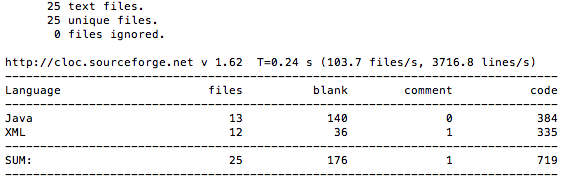
\includegraphics[width=0.8\textwidth]{images/cloc-proto.png}
  \caption{CLOC results for the prototype project}
\end{figure}
\begin{figure}[H]
  \centering
  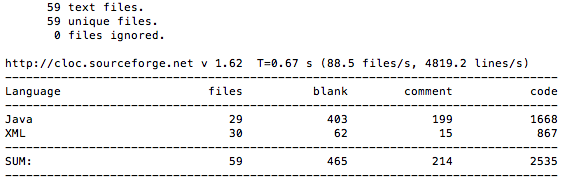
\includegraphics[width=0.8\textwidth]{images/cloc-alpha.png}
  \caption{CLOC results for the alpha project}
\end{figure}
\begin{figure}[H]
  \centering
  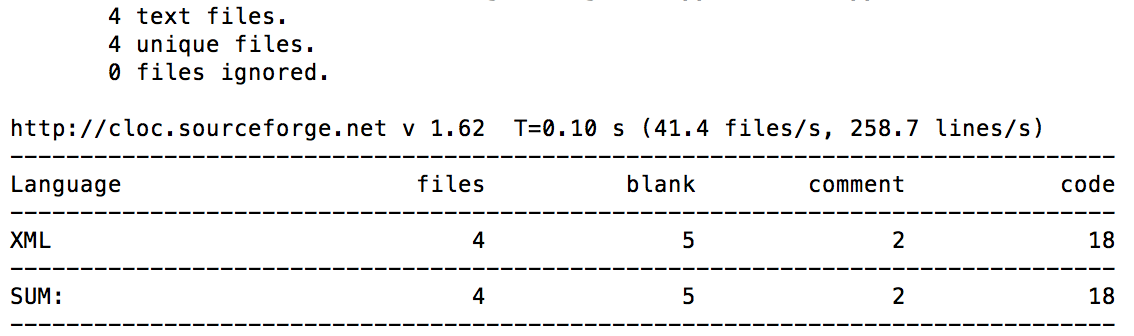
\includegraphics[width=0.8\textwidth]{images/cloc-blank.png}
  \caption{CLOC results for a blank new project}
\end{figure}
\end{document}
